\documentclass[a4paper]{extarticle}
\usepackage[utf8]{inputenc}
\usepackage[a4paper, margin=1in]{geometry}

\usepackage{amssymb}
\usepackage{amsmath}
\usepackage{enumitem}
\usepackage{tcolorbox}
\usepackage{fancyhdr}
\usepackage{graphicx}
\usepackage{float}

\setlength{\parindent}{0em}
\setlength{\parskip}{0.4em}

\definecolor{theoremblue}{RGB}{1, 73, 124}
\definecolor{corollaryblue}{RGB}{70, 143, 175}
\definecolor{exampleblue}{RGB}{137, 194, 217}

\newtcolorbox{tbox}{colback=theoremblue!20,colframe=theoremblue,
boxrule=0pt,arc=0pt,boxsep=2pt,left=2pt,right=2pt,leftrule=2pt}

\newtcolorbox{cbox}{colback=corollaryblue!20,colframe=corollaryblue,
boxrule=0pt,arc=0pt,boxsep=2pt,left=2pt,right=2pt,leftrule=2pt}

\newtcolorbox{ebox}{colback=exampleblue!20,colframe=exampleblue,
boxrule=0pt,arc=0pt,boxsep=2pt,left=2pt,right=2pt,leftrule=2pt}

\title{EnpRisk - Lecture Notes Week 8}
\author{Ruben Schenk, ruben.schenk@inf.ethz.ch}
\date{\today}

\pagestyle{fancy}
\fancyhf{}
\rhead{ruben.schenk@inf.ethz.ch}
\rfoot{Page \thepage}
\lhead{EnpRisk - Lecture Notes Week 8}

\begin{document}

\maketitle

\section{150 Years of Society, Economy and Technology}

\subsection{Overview}

\begin{figure}[H]
    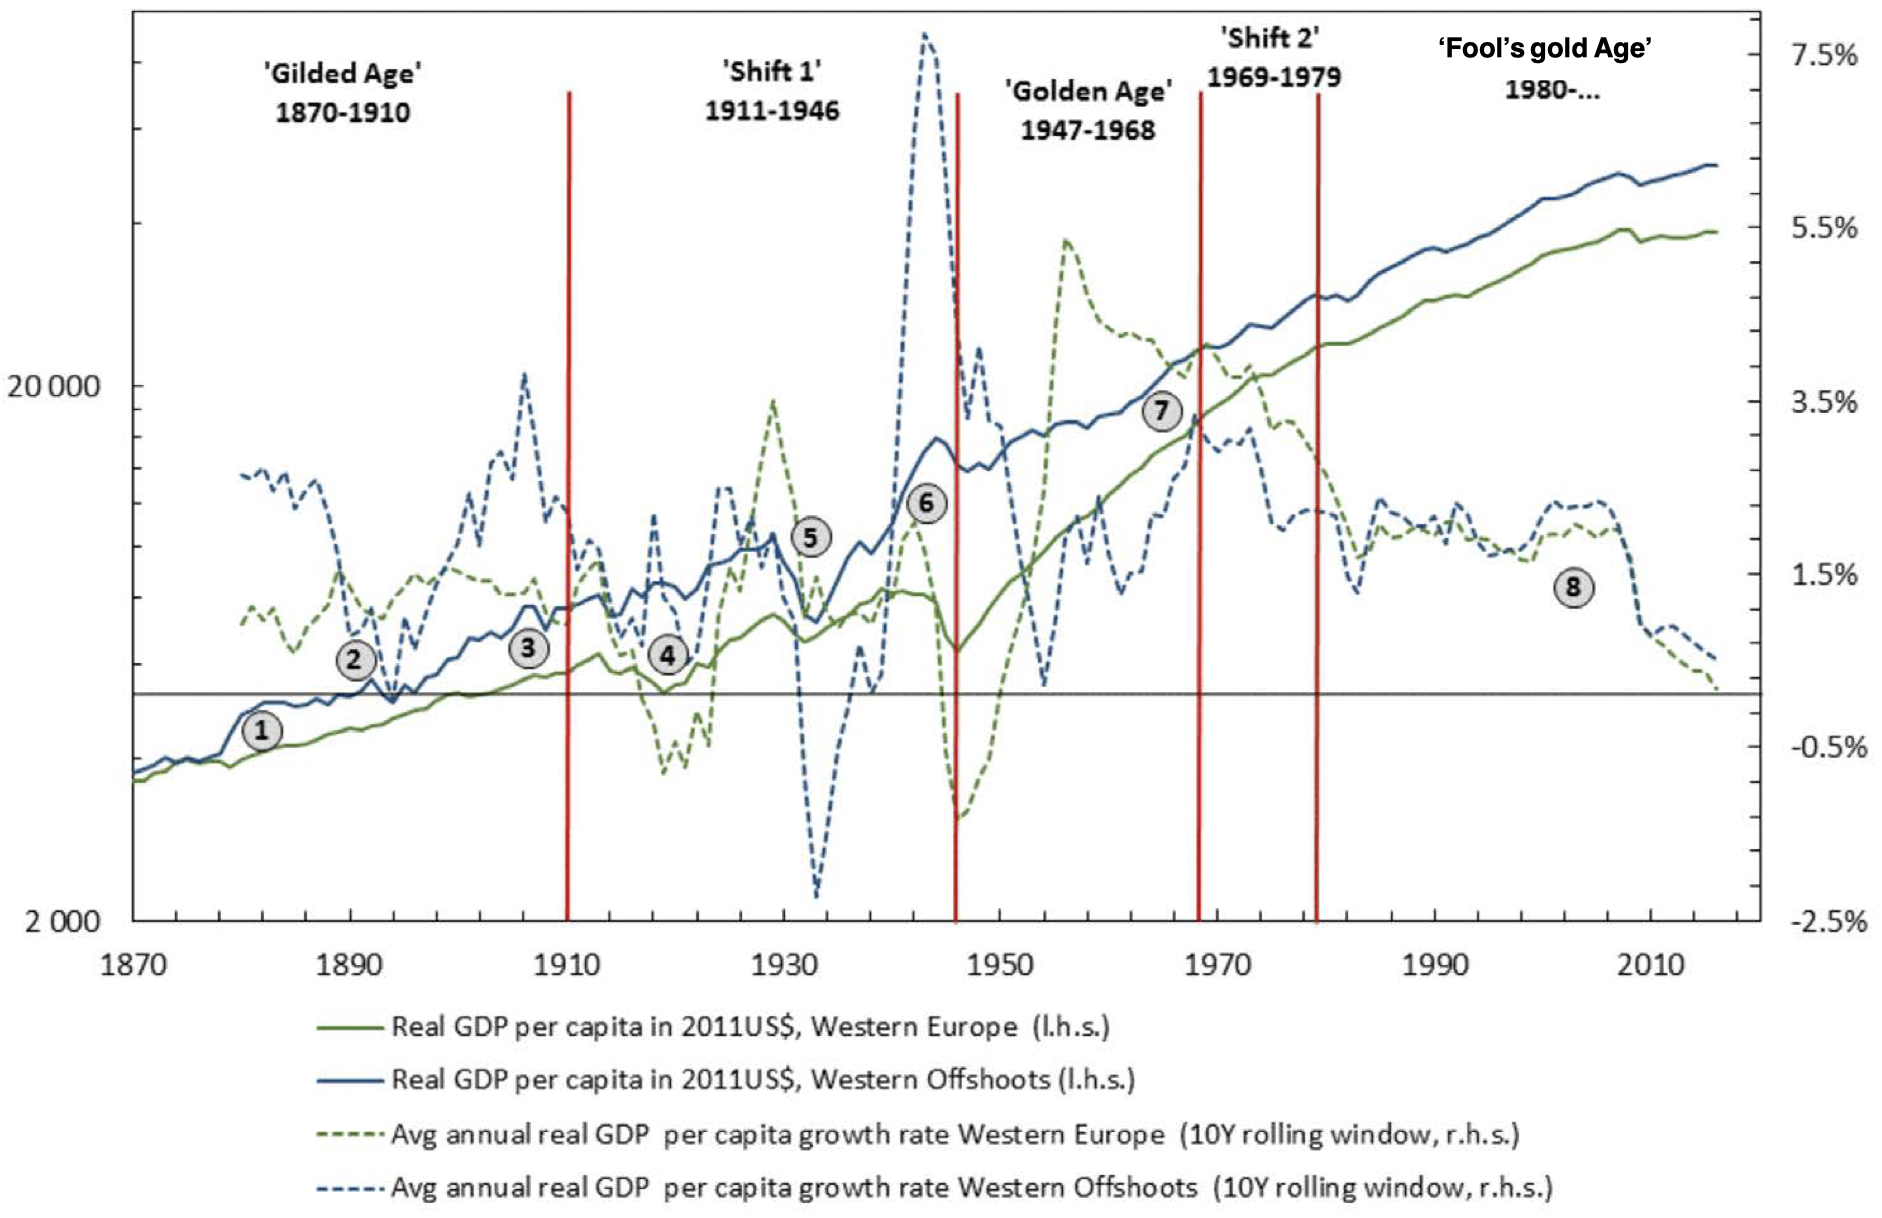
\includegraphics[width=15cm]{../images/EnpRisk_Fig8-1}
    \centering
\end{figure}

When one structural economic regime passes into another, the economic system goes through a shift. Because each shift experiences the end of one era and the beginning of another, it always comes with \textit{geopolitical, financial and economic disruption and distress.}

However, during these shifts, also reform takes place, where the seed are planted from which a new structural regime takes root.

\subsection{The Gilded Age (1870-1910)}

\textit{"A gilded object looks shiny from the outside. But when you scratch the surface, the underlying material is revealed, and it is certainly not golden."}

In short, the \textbf{gilded age} is described by the following points:

\begin{itemize}
    \item Era of rapid expansion of heavy industries and infrastructure
    \item Accelerated innovation from the \textit{Technological Revolution} led to interconnected growth such as telegraphs, railroads, transatlantic ship routes, etc.
    \item First wave of \textit{globalization:} Rise of the "haute finance", centered around the Gold Standard, with the British Pound as reserve currency
    \item The stock market, during these times, was solid, with high earning qualities and a strong underlying economic growth
    \item The balance of power, between the newly created nation states, guaranteed geopolitical stability. This prevented the occurrence of any wars between the Great Powers ("Belle Epoque" in France)
\end{itemize}

However, \textit{inequalities were at a historical high:}

\begin{itemize}
    \item Urbanization and migration led to an oversupply of labor in the cities
    \item There was a stagnation of real wages
    \item There was a decline of the proportion of GDP going to labor
\end{itemize}

This robber baron capitalism and winner-takes-it-all markets created monopolies: The fruits of progress stayed in the hands of the happy few.

In general, the Gilden Age was a period of wild financial and economic expansion with a \textit{lack of institutions and regulations} to smoothen boom and fight bust. As a result, we see multiple cycles of boom, panic and depression:

\begin{itemize}
    \item 8 years of overinvestment and speculation, and a railroad boom after the end of the American Civil War (1865) ended in the panic of 1873
    \item This was followed by the \textit{Long Depression} which lasted until 1879
    \item A new boom started, pushed by the Technological Revolution, which lasted until the panic of 1893, ensued by another depression which lasted until 1897
    \item This was then followed by another boom, which ended in a massive banking crisis in 1907
\end{itemize}

Economic policymakers want to achieve three goals:

\begin{enumerate}
    \item Open their country's economy to international flows of capital to allow the nation's citizen to diversify their investments abroad.
    \item Follow an independent monetary policy to stabilize their economy and support employment in times of need.
    \item Have a fixed foreign exchange rate which brings stability and trust in the international trade and investment.
\end{enumerate}

However, the \textit{trilemma of international finance} states you can only have two out of the three:

\begin{figure}[H]
    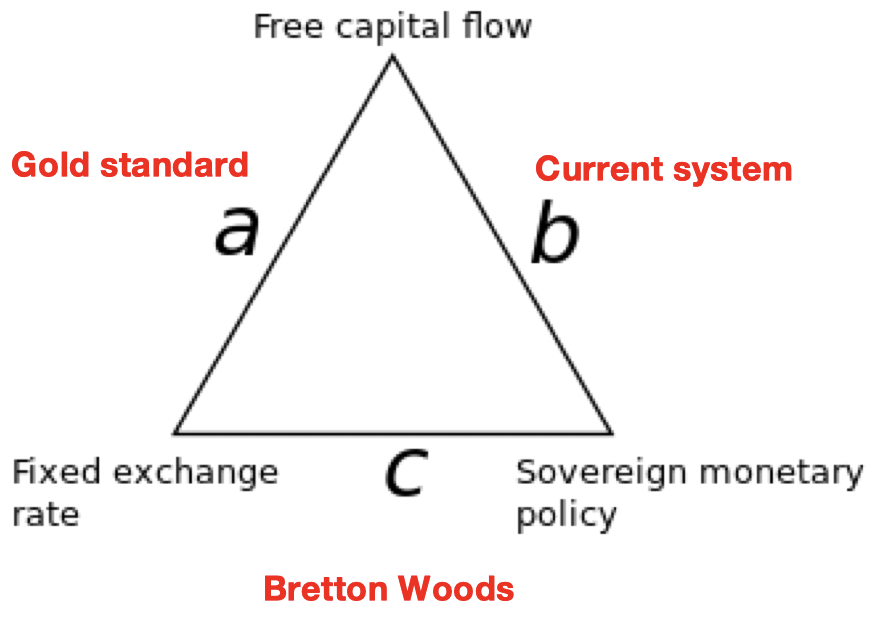
\includegraphics[width=9cm]{../images/EnpRisk_Fig8-2}
    \centering
\end{figure}

\subsection{The First Shift (1911-1946)}

During the \textbf{first shift} (1911-1946), there was an institutional reform with Roosevelt's New Deal (1933-1939):

\begin{itemize}
    \item Stabilizing the banking system through bank reform acts
    \item Suspension of the Gold Standard, with freely floating US Dollar and increase of money in circulation by Federal Reserve
    \item Increase transparency in the stock market by mandatory publication of balance sheet, profit and loss statements, etc.
    \item Public works and relief: Hire unemployed to build schools, municipal buildings, waterworks, sewers, streets, etc.
    \item Social security act establishing a permanent system of pensions, unemployment insurance, etc.
    \item National Labor Relations Act: guaranteed workers the right of collective bargaining through unions
    \item Fair Labor Standards Act set a maximum of 44 hours of work per week and minimum wages, child labor under 16 was forbidden
    \item Wealth Tax Act: Redistribute wealth by imposing a tax of 79\% on incomes over 5 million USD
\end{itemize}

Finally, in the summer of 1944, 730 representatives of 44 countries gathered at the \textbf{Bretton Wood} conference with the goal of \textit{redesigning the international monetary system.} The new system should:

\begin{itemize}
    \item Replace the monetary chaos of interwar period with a new international system that would support trade through stable exchange rates
    \item Free trade was preferred to free capital flows, especially in short-term "hot money" flows and capital flight. As such, it was explicitly recognized that countries need to impose capital controls
    \item Each country could still follow an independent monetary policy to fight recession and stimulate employment
\end{itemize}

\end{document}